\chapter{Classifier}
\section{Overview}
The classifier`s task is to solve the following problem: given a vector of 1024 attributes, determine which feature this vector represents. To solve this problem, the classifier must identify patterns in the attribute vectors extracted from features of the same type, and use this to distinguish them from other features, much like a fingerprint. 
Figure \ref{fig:spark_problem} shows a visualisation of these ``fingerprints" in a spark diagram. This diagram shows each 1024 attributes extracted from 20 features. Each row represents a feature, and each vertical bar represents the value of that attribute of that feature
Figure \ref{fig:spark_solution} shows how subtle patterns can be found within these ``fingerprints" that can be used to identify the feature they were extracted from
\begin{figure}[H]
    \centering
    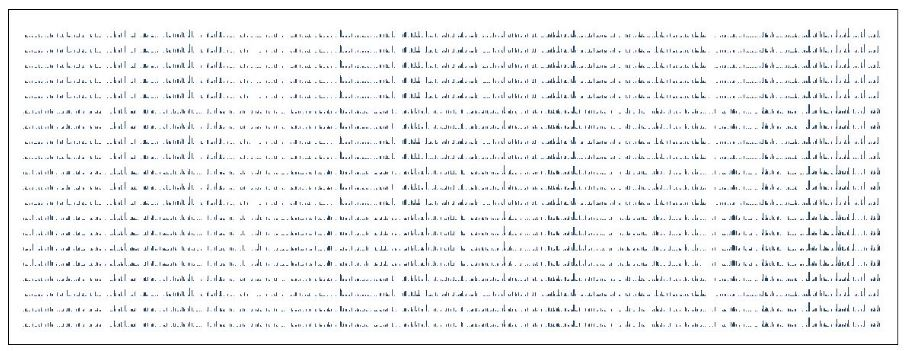
\includegraphics[width=\textwidth]{figs/8/spark_diagram}
    \caption{A 20-feature spark diagram}
    \label{fig:spark_problem}
\end{figure}

\begin{figure}[H]
    \centering
    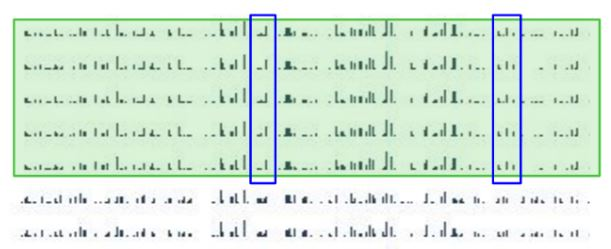
\includegraphics[width=\textwidth]{figs/8/spark_solution}
    \caption{ A subtle pattern that distinguishes vectors of Trees (highlighted in green) from the vectors of all other features}
    \label{fig:spark_solution}
\end{figure}

To achieve this, the classifier must be able to perform two key functions:
\begin{itemize}
    \item Learn - used to train the classifier via supervised learning
    \item Guess - used to receive the classifier's predictions regarding the class of an attribute vector
\end{itemize}

\section{Background Research}
There are a number of classification algorithms available, each with their strengths and limitations. For our problem, the classification algorithm must be capable of:
\begin{itemize}
    \item Handling high-dimensional input
    \item Learning quickly
    \item Learning iteratively
    \item Identifying a dynamic number of classes
\end{itemize}

\newpage
\subsection{Perceptron}
A binary perceptron provides a simple approach for determining if a given input belongs to a specific class or not. Given inputs 1 to N $x_n$, multiply each input by its corresponding weight 1 to N $w_n$, and if the sum of this reaches a threshold $T$, the input is predicted to belong to the class \citep{perceptron} (See figure \ref{fig:perceptron_img}).
$$ 
x \text{ belongs to class} = 
\begin{cases}
\mbox{True} &
\sum_{n=1}^{N} (x_n \cdot w_n) \geq T \\
\mbox{False} & \text{otherwise}
\end{cases}
$$

\begin{figure}[H]
    \centering
    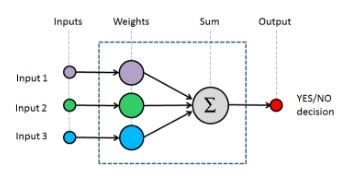
\includegraphics{figs/8/perceptron_img}
    \caption{Perceptron Structure}
    \label{fig:perceptron_img}
\end{figure}

Strengths:
\begin{itemize}
    \item Quick and easy to implement
\end{itemize}
Limitations:
\begin{itemize}
    \item Can only provide linear solutions
    \item Requires significant training data to make accurate predictions
    \item Ineffective with high-dimensional input
    \item Can’t solve the XOR problem
\end{itemize}
Time Complexity:
\begin{itemize}
    \item Learn: O(c) - but extensive training required
    \item Classify: O(c) - but poor accuracy unless sufficiently trained
\end{itemize}
\citep{perceptron_2}

\subsection{Neural Network}
A neural network consists of a number of perceptrons, arranged in layers such that the output from one perceptron feeds into the input of the next perceptron. The n-dimensional input is passed to m perceptrons in the input layer and fed through the neural network. Upon reaching the output layer, probabilities are provided for the input belonging to each class known by the network. If the prediction is incorrect, the process is reversed and the weightings of each node are modified accordingly \citep{neuralnetwork} (See diagram below \ref{fig:neuralnetwork_img}). 

\begin{figure}[H]
    \centering
    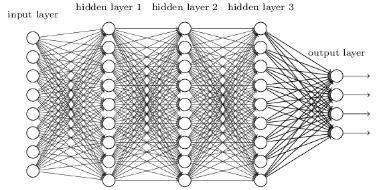
\includegraphics{figs/8/NN_img}
    \caption{Neural Network structure}
    \label{fig:neuralnetwork_img}
\end{figure}

Strengths:
\begin{itemize}
    \item Can provide linear and nonlinear solutions
    \item Requires less training than the perceptron
    \item Can achieve high levels of accuracy
    \item Provides probability estimates
\end{itemize}

Limitations:
\begin{itemize}
    \item Still requires a large amount of training data
    \item Ineffective with high-dimensional input
    \item Has a complex design that requires significant fine-tuning
    \item Can only classify a static number of classes
\end{itemize}

Time Complexity:
\begin{itemize}
    \item Learn: O($N^{L}$) - where N is the number of input nodes and L is the number of layers
    \item Classify: O($N^{L}$) - where N is the number of input nodes and L is the number of layers
\end{itemize}

\subsection{Support Vector Machine (SVM)}
An SVM maps n-dimensional input into an n-dimensional space, and find planes that separate each class while maximising the distance between them. Then, given some n-dimensional input, it predicts the class of the input based on which side of the separating plane it falls on \citep{svm} (see figure \ref{fig:svm_img}) 

\begin{figure}[H]
    \centering
    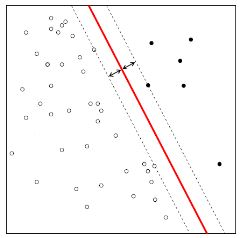
\includegraphics{figs/8/linear_svm}
    \caption{Diagram of SVM showing plane separating two classes}
    \label{fig:svm_img}
\end{figure}

Strengths:
\begin{itemize}
    \item Can provide linear and nonlinear solutions
    \item Effective with high-dimensional input
    \item Requires significantly less training than Neural Networks or Perceptrons
    \item Supports iterative learning
\end{itemize}

Limitations:
\begin{itemize}
    \item Unable to directly provide probability estimates
    \item Performs poorly as the number of classes increases
\end{itemize}

Time Complexity:
\begin{itemize}
    \item Learn: O(N) - where N is number of data entries
    \item Classify: O(n) - where n is the number of classes
\end{itemize}

\section{Design}
\subsection{Design Decisions}
\subsubsection{Classification Algorithm}
The SVM was selected since it best suited the needs of the project:
\begin{itemize}
    \item It requires little training data, which improves the system’s usability
    \item It handles high-dimensional input effectively, which is essential since the input has 1024 dimensions
    \item It supports iterative learning across a dynamic number of classes, which are strict requirements of the system
\end{itemize}

A number of machine learning libraries are available in python, but scikit-learn was selected as it provides a range of well implemented and well documented classification algorithms for free \citep{scikit-learn}.

One drawback of the SVM is that it can’t directly probability estimates. While these can be calculated based on the distance of a point to its surrounding separating planes, these values proved to be inaccurate, often contradicting the actual prediction of the SVM.  However, the implementation of Olivia allows probabilities to be obtained using contextual classification. By default, the attributes extracted by Olivia are based on the centre pixel of a 256x256 image, using the surrounding 192x192 pixels as context, and ignoring the outer 32 pixels on each side.

\begin{figure}[H]
    \centering
    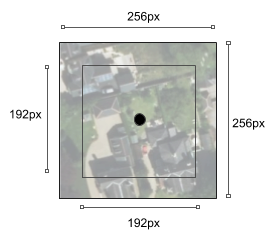
\includegraphics{figs/7/tile_range}
    \caption{Default image extraction zone}
\end{figure}

Contextual classification is the process of shifting Olivia’s focus point to 9 different positions in the image, such that every pixel is \textit{included as context}. This achieves 9 unique classifications per image, allowing probability estimates to be calculated from the results of these classifications.

\subsubsection{Linear SVM vs Non-Linear SVM}
There are a number of varieties of SVM, including linear and nonlinear SVMs. Linear SVMs separate classes with a linear plane (\ref{fig:linear_svm}), while non-linear SVMs use a Kernel function to transform each point and map them into a new space, in which a linear separation plane is found. The transformation makes it equivalent to using a curved line in the original input space, enabling higher accuracy and providing a solution to problems that can’t be solved with a Linear SVM. (\ref{fig:non_linear_svm}). 
\begin{figure}[H]
    \centering
    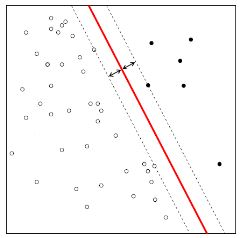
\includegraphics{figs/8/linear_svm}
    \caption{Linear SVM}
    \label{fig:linear_svm}
\end{figure}

\begin{figure}[H]
    \centering
    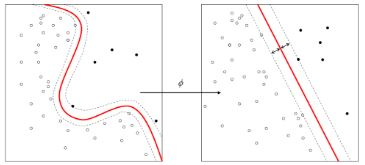
\includegraphics{figs/8/non_linear_SVM}
    \caption{Non-Linear SVM}
    \label{fig:non_linear_svm}
\end{figure}

By developing a test that mimics the use of the classifier within the system, the performances of both flavours was compared, allowing for the optimal approach to be selected. The following test was devised:
\begin{itemize}
\item 4 feature classes
\item 5 entries per class (20 data entries in total)
\item 4 entries per class given as training data.
\item Asked to predict the final entry
\item Entries rotated round-robin-style for a total of 20 tests
\item Overall accuracy calculated by percentage of correct predictions
\end{itemize}
In this test, the linear SVM had an top-1 accuracy of 80\%, while the non-linear SVM’s accuracy was only 65\%. This is likely due to the large-dimensional input, which increases the chances of a linear separating plane existing, allowing the linear SVM to perform well, while significantly more fine-tuning and training data would be required for an accurate nonlinear plane to be formed. Therefore, a linear SVM was selected.

\subsubsection{1vAll vs 1v1}
Another variety of SVM to consider is 1vAll or 1v1. The 1vAll SVM separates each class from all other classes using a single separating plane (\ref{fig:1vAll}, producing N SVMs, whereas a 1v1 SVM separates each class from each other class, resulting in $\frac{N(N-1)}{2}$ planes where N is the number of classes (\ref{fig:1v1}). 
\begin{figure}[H]
    \centering
    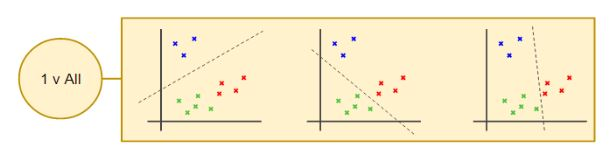
\includegraphics{figs/8/1vall_svm}
    \caption{1 vs All SVM - separating planes}
    \label{fig:1vAll}
\end{figure}
\begin{figure}
    \centering
    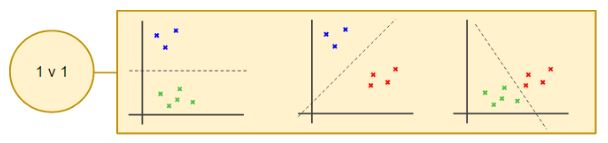
\includegraphics{figs/8/1v1_svm}
    \caption{1 vs 1 SVM - separating planes}
    \label{fig:1v1}
\end{figure}

Following the same test as above, 1v1 achieved top-1 80\% accuracy whereas 1vAll only achieved 55\% accuracy. 
However, 1v1 scales poorly as the number of classes increases, requiring (n-1)! separating planes to be calculated, compared to 1vAll which only requires n.
Overall the accuracy of the system was prioritised over its speed, so the 1v1 approach was selected.

\subsubsection{ Iterative learning: Partial Fit vs Knowledge Persistence}
A concrete requirement for the system is its ability to learn iteratively, allowing users to provide training data in increments rather than one large batch.

SVM has a ``partial fit” function, whereby the separating planes can be incrementally modified as the SVM’s knowledge increases. However, since the user would likely train the classifier one class at a time, providing batches of data belonging to that class, this was shown to cause the SVM to overfit for the class it was most recently trained with, significantly impacting its accuracy.

An alternative solution was to store all of the training data passed to the SVM. As new training data is provided, it can combine this with all previous data, and perform a regular fit. This not only eliminates the problem of overfitting, but also allows control over the SVMs knowledge, such that information can be un-learned by removing the entry from memory.
The cost to this approach is a memory requirement of the system that increases with the SVMs training. However, if this becomes an issue a remote database could be used instead.
Therefore, the knowledge persistence approach was selected.

\section{Implementation}
\subsection{Class Lookup Table}
The class lookup table provides an auxiliary function for converting human-readable feature names to SVM-useable ID numbers. This is achieved by a lookup table that maps feature_name to class_id. The table is implemented as a CSV file, and the user can dynamically add/remove entries to/from this table via the user interface. A unique class ID number is generated whenever the user adds a new class. If the user removes a class, training data belonging to that file is also removed from the SVM’s memory. 

\subsection{Classifier Knowledge Persistence}
The SVM’s knowledge persistence is again implemented using a CSV file. 
On start-up, it reads all previous training data from the CSV file into two arrays: attribute\_vectors and class\_ids. If it contains no previous training data, it uses the default training data file, containing data for 4 default classes: tree, road, building and house. If this file doesn’t exist, the arrays are left empty.
As additional training data is provided, it is appended to the two arrays. On shutdown, all data in the arrays is written back to the CSV in the format: [class\_id, attribute\_vector].

\subsection{Learn Function}
The learn function, along with the guess function, make up the core functionality of the classifier. The learn function’s implementation is as follows:
\begin{itemize}
    \item On start-up, reads all data from storage into the attribute\_vectors and class\_ids arrays
    \item Accepts a dictionary of [image url : attribute vector] and an array of corresponding feature names 
    \item Uses the Class Lookup Table to convert the feature name to its class ID
    \item Appends the new attribute vectors to the attribute\_vectors array, and the new class IDs to the class\_ids array
    \item If the data in the arrays only corresponds to a single class, returns a message informing the user that data for at least two classes is required before the SVM can fit 
    \item Else, performs a fit using all data provided and returns a success message
\end{itemize}

\subsection{Guess Function}
The guess function is implemented as follows:
\begin{itemize}
    \item On start-up, reads all data from storage into the attribute_vectors and class_ids arrays
    \item Accepts a dictionary of [image url : attribute vector]
    \item If the SVM hasn’t yet received sufficient data to perform a fit, returns an error message informing the user that further training across additional classes is required
    \item Else, predicts the class ID of each attribute vector
    \item Uses the Class Lookup Table to convert the class ID to a human-readable feature name
    \item Returns a dictionary of [image url : predicted feature name]
\end{itemize}

\section{Testing}
\subsection{SVM Testing}
Regression testing was used to ensure the guessing accuracy of the SVM didn’t deviate when trained on the same sets of data. This ensures that the library used performs consistently with our training data while learning iteratively using several refits.

Unit testing was used to test the knowledge persistence of the SVM. Firstly, the test verified that the SVM used previous data from the CSV file on startup. Secondly, it tested that, if this file doesn’t exist, the default training data is used. Finally it tested that, new training data is provided via the learn function, this data is correctly written to the CSV file, even when the SVM is shut down unexpectedly.
\subsubsection{Class Lookup Table Testing}
Unit testing was used to check all aspects of the Class Lookup Table’s functionality.

Firstly, it was ensured that classes could be added or removed from the table correctly. Additionally, upon removing a class, the test ensured that all corresponding data entries were removed from the SVM’s memory. 

Secondly, the functions for finding a class ID from its name and vice versa were tested. The test ensured these functions behaved consistently as new classes were added and removed.
\subsubsection{Endpoint Testing}
The endpoints of the classifier microservice were tested to ensure they behaved correctly with valid input, and returned an appropriate error message when given invalid input.

Unit tests were developed to ensure the Learn Endpoint responded correctly to the following cases:
\paragraph{Valid Input\\}
\tab Returns Success
\paragraph{Invalid Input: the number of vectors doesn’t match the number of class IDs\\}
\tab Returns Length Mismatch Exception
\paragraph{Edge case: the classifier has only been given training data for a single class\\}
\tab Returns Not Ready To Predict Message

Similar tests were developed for the Guess Endpoint:
\paragraph{Valid Input\\}
\tab Returns Success
\paragraph{Invalid input: list of vectors is empty\\}
\tab Returns Empty List Exception
\paragraph{Edge case: the classifier has only been given training data for a single class\\}
\tab Returns Not Ready To Predict Message

\section{Limitations}
The design decisions and implementation of the classifier result in the following limitations:

Firstly, the SVM algorithm scales poorly as the number of classes increases, especially when using the 1v1 variety, as significantly more separating planes must be computed. Additionally, further training data is often required in this case as the space between classes typically  reduces. However, this effect is reduced due to the high-dimensional data used by the system. 

Secondly, storing all training data in a CSV file adds an additional memory requirement to the system. Each data entry, consisting of a class ID and 1024 attribute values, is approximately 5kb in size. Alone this doesn’t pose as a significant problem, but since there is no confirmed upper boundary for the quantity of training data that would be used, there is the possibility of this becoming a significant overhead. If this becomes the case, the data would need to be moved to a remote database.

Finally, by fitting the SVMs separating planes using all learnt data while using a 1v1 variety, this could significantly increase the time taken to fit the graph. However, upon testing the time taken for a 1v1 SVM to fit its separating planes based on 10,000 data entries, this only took approximately 5 seconds, so is unlikely to be a problem.

\section{Evaluation}
Overall, the design and implementation of this classifier has ensured the key requirements of the system are met. 
The SVM algorithm is capable of efficiently handling high-dimensional data, requires minimal training from the user, and provides accurate predictions. Through the implementation of knowledge persistence, it is capable of learning iteratively, the number of classes can be modified dynamically and its knowledge can be easily managed.
One flaw of the SVM is its inability to directly give probabilities, but the use of contextual classification provided a workaround to this, albeit somewhat less precise.
However, while adaptations made to the classifier optimise its accuracy, functionality and utility, this comes at the cost of a design that scales poorly as the number of classes and training data increases.
